\chapter{The simulator}\label{ch:simulator}

The purpose of the simulator is to visualize the movement of a simple snake robot model progressing according to a predefined path and obstacles in the environment.

This chapter aims at describing how the simulator is structured and can be used, as well as explaining particular code snippets in more detail. Moreover, it provides an overview of how the mathematical background is applied.
%-----------------------------------------------------------------------------------
%-----------------------------------------------------------------------------------

\section{Simplifications and limitations}

Expressing the complete dynamics of the system includes explicitly finding the part of the joint torques that are not directly applied to the robot joints, but rather a force acting on the external obstacles. In other words, the torque would have to be separated in a component belonging to the constraint- or propulsion space and a component that belongs to the shape space (see \ref{subseq:snakeHPFC}).

This challenge, combined with a strict time schedule, has led to a simplification in the development of the simulator. In the simulator, the movement of the robot is first calculated under the assumption that no obstacle is present. To account for this, the interaction forces are implicitly considered through mapping to the allowable position space. This means that if the robot is in contact with the environment, the joint velocities are influenced accordingly and thus also the joint angles. The consequences of the simplification are discussed in chapter \ref{ch:discussion}.

Like in any computer simulation, the time is discretized. This leads to inaccuracies, especially for fast motions. To minimize the effect of the simplification, the sampling time may be decreased. 

Furthermore, the projection onto the desired path assumes that the robot is sufficiently close to the path to get back to it. The calculated desired angles for joints very far away from the path might therefore not lead to advantageous behaviour. The projection also assumes that the links of the robot are chronologically aligned along the path. This means that if the robot is for instance curled up, the projection will fail to align the robot.


%-----------------------------------------------------------------------------------
%-----------------------------------------------------------------------------------

\section{Program flow}

The program flow is illustrated in the diagram figure \ref{fig:prog_flow}. The blue rectangles represent functions, and the data connected to the outgoing arrows are computed output variables. From the diagram, it is noticeable that the program runs in a loop after initialization, constantly controlling the robot towards the path while adapting to its environment (the obstacles).

Initialization is performed based on the given snake robot and obstacle configurations. Furthermore, the joint acceleration $\mathbf{\ddot{q}}$ of the robot is found by solving the dynamics equation (\ref{eq:eom_qdd}), where the joint torque $\boldsymbol{\tau}$ is calculated by the computed torque control (\ref{eq:controllaw}). The control reference is based on deviation from the desired trajectory (see section \ref{sec:pathproj}). Joint velocities $\mathbf{\dot{q}}$ and angles $\mathbf{q}$ are deduced from $\mathbf{\ddot{q}}$ using Euler integration.

Whenever the robot is in contact with one or more obstacles, the joint velocities are projected onto the allowable position space using the intersect of all $\prescript{j}{ap}{P}$, explained in \ref{subseq:HPFC}.

\begin{figure}
    \centering
    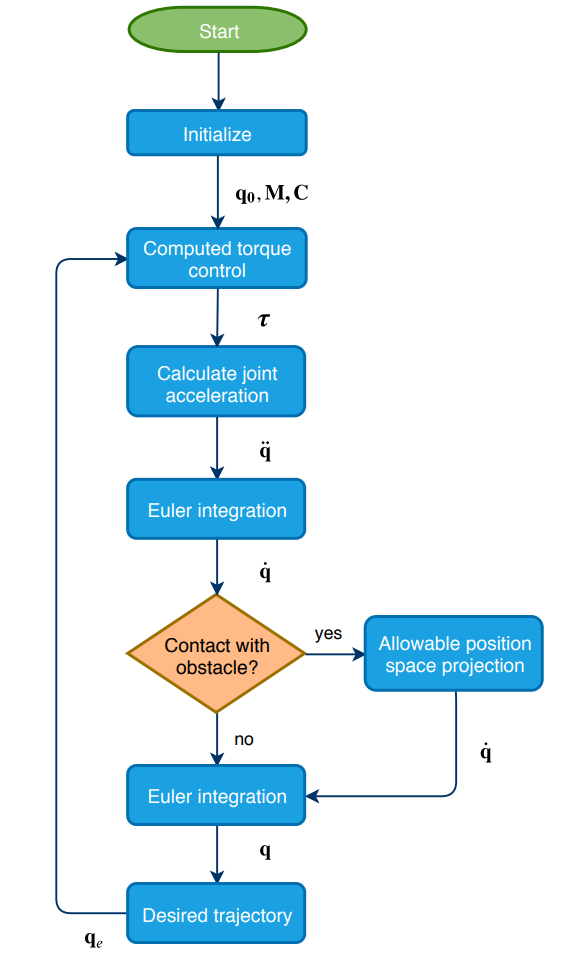
\includegraphics[width=0.75\textwidth]{figures/sysflow.PNG}
    \caption{Program flow diagram}
    \label{fig:prog_flow}
\end{figure}


\section{User guide}

The user can adjust parameters related to the specifications of the snake robot, obstacles in the environment, the desired path the robot should attempt to follow and control parameters. A snapshot of the visual output of these variables are shown in figure \ref{fig:sim_vis}.

\begin{figure}
    \centering
    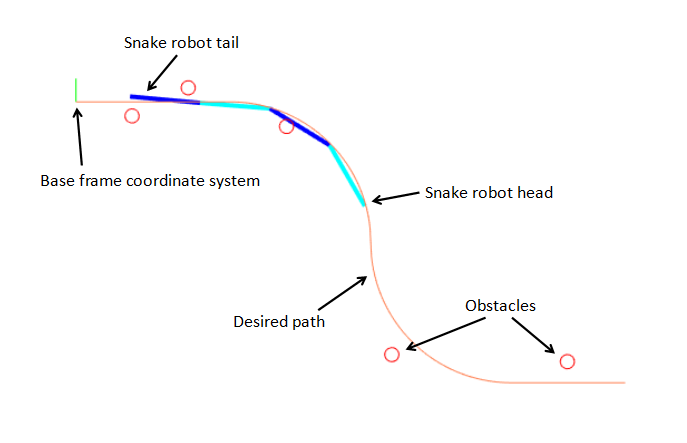
\includegraphics[width=0.9\textwidth]{figures/sim_vis.png}
    \caption{Visual output of simulation}
    \label{fig:sim_vis}
\end{figure}

Once the variables are adjusted in the respective files, the \\ \texttt{initialization.m} script can be run. For a specific configuration, this initialization only has to be run once for every time MATLAB is started. The variables will then end up in the MATLAB workspace and the simulation can be run for a wished number of times. Variables that do not change the dynamics properties of the robot can be redefined without running the whole initialization over.

The user definable variables are summarized in table \ref{tab:sim_userparams}.

\begin{table}
\centering
    \begin{sideways}
    \begin{tabular}{|c|c|c|c|c|}
        \hline
        \textbf{\small{Parameter description}} & \textbf{\small{Parameter name}} & \textbf{\small{Filename}} & \textbf{\small{Datatype}} & \textbf{\small{Unit}}\\
        \hline \hline
        \footnotesize{Number of links} & \texttt{n} & \texttt{init\char`_snake.m} & Integer & \\
        \hline
        \footnotesize{Link length} & \texttt{l}  & \texttt{init\char`_snake.m} & Float & $m$\\
        \hline
        \footnotesize{Link mass} & \texttt{m} & \texttt{init\char`_snake.m} & Float & $kg$\\
        \hline
        \footnotesize{Initial robot configuration} & \texttt{q0} & \texttt{init\char`_snake.m} & Array of floats & $rad$\\
        \hline
        \footnotesize{Number of obstacles} & \texttt{num\char`_obstacles} & \texttt{init\char`_obstacles.m} & Integer & \\
        \hline
        \footnotesize{Obstacle coordinates} & \texttt{obstacle\char`_coords} & \texttt{init\char`_obstacles.m} & 2D array of floats & $m$\\
        \hline
        \footnotesize{Obstacle safety radius} & \texttt{obstacle\char`_radius} & \texttt{init\char`_obstacles.m} & Float & $m$\\
        \hline
        \footnotesize{Proportional control gain} & \texttt{kp} & \texttt{init\char`_control.m} & Float &\\
        \hline
        \footnotesize{Derivative control gain} & \texttt{kd} & \texttt{init\char`_control.m} & Float &\\
        \hline
        \footnotesize{Torque saturation limit} & \texttt{max\char`_tau} & \texttt{init\char`_control.m} & Float & $Nm$\\
        \hline
        \makecell{\footnotesize{Number of individual }\\\footnotesize{functions defining the path}}  & \texttt{num\char`_sections} & \texttt{init\char`_path.m} & Integer & \\
        \hline
        \makecell{\footnotesize{Intersection point of path}\\\footnotesize{functions along x}}  & \texttt{section\char`_partition} & \texttt{init\char`_path.m} & Array of floats & $m$ \\
        \hline
        \footnotesize{Functions defining the path}  & \texttt{curve} & \texttt{init\char`_path.m} & Set of functions & $m$\\
        \hline
    \end{tabular}
    \end{sideways}
    \caption{User adjustable simulator parameters}
    \label{tab:sim_userparams}
\end{table} 


\section{Program code summary}

The whole simulator is made, and to be executed, in MATLAB. The symbolic toolbox \cite{matlabsymbolic} has been used to generalize the code and make it adaptable to an n-link snake robot. The whole code can be accessed through \hl{...}

The values $l$, $m$, $n$, $N$, $K_p$, $K_d$, $\mathbf{q}$ and $\mathbf{\dot{q}}$ from chapter \ref{chapter:theory} are globally defined and accessible for scripts/functions that might need them.

\subsection{Dynamics functions}

The dynamics, more particularly the matrices $M$ and $C$ from (\ref{eq:eom}), are generated symbolically in the script \texttt{init\char`_dynamics.m}.
As a result of the use of symbols, the matrices can be used as functions with the joint angles and velocities as input parameters.


\subsection{Kinematics functions}\label{subseq:kinfunc}

The script \texttt{init\char`_kinematics.m} generates the transformation matrices from (\ref{eq:transformationmatrix}), defining the relation from base to every link endpoint. These matrices are -- equivalent to the dynamic matrices from last section -- expressed with symbols. Additionally, functions for generating the rotation matrix around the z-axis, \texttt{Rz\char`_func(theta)}, and translation matrix in the x- and y direction, \texttt{D\char`_func(x\char`_dist, y\char`_dist)} are defined.

%-----------------------------------------------------------------------------------------
%-----------------------------------------------------------------------------------------

\subsection{Contact Jacobian function}\label{subseq:Jcfunc}
The symbolic expression of the contact Jacobians is calculated in \\ \texttt{init\char`_contact\char`_jacobians.m}. As there can be a maximum of one obstacle touching each link, there is one general contact Jacobian calculated per link.

\begin{itemize}
    \item \textbf{Lines 2-8:} The position of the contact point in the base frame expressed by the joint variables is extracted from the homogeneous transformation matrix (see section \ref{sec:kin}).
    \item\textbf{Lines 9-12:} Partial differentiation of the position of the contact point with respect to the generalized coordinates to obtain the contact Jacobian.
    \item \textbf{Line 14:} All contact Jacobians are stacked in a 3-dimensional matrix.
\end{itemize}

The variable \texttt{q} represents the vector of generalized coordinates, and \\ \texttt{Rz\char`_func(theta)} and \texttt{D\char`_func(x\char`_dist, y\char`_dist)} are previously defined functions, see \ref{subseq:kinfunc}.

\lstinputlisting[firstline=23, lastline=37]{Simulator_code/init_contact_jacobians.m}

%-----------------------------------------------------------------------------------------
%-----------------------------------------------------------------------------------------

\subsection{Projection function}

The projections are calculated in the function \texttt{calc\char`_projections.m} based on the functions for the contact Jacobians. 

In the following code snippet from the function, contact on link \texttt{i} is already established and the corresponding projection matrices are to be found.

\begin{itemize}
    \item \textbf{Line 2:} The variable \texttt{q(n+2+i,k)} corresponds to the generalized coordinate $d_{c,i}$ (see (\ref{eq:q2})).
    \item \textbf{Lines 3-4:} The contact Jacobian with current $\mathbf{q}$-values from simulation. The function used is explained in \ref{subseq:Jcfunc}.
    \item \textbf{Lines 5-6:} Projection matrices from (\ref{eq:proj_mtrices}).
    \item \textbf{Lines 7-8:} Projection matrices are stacked.
\end{itemize}


\lstinputlisting[firstline=73, lastline=80]{Simulator_code/calc_projections2.m}

Seeing as there might be more than one contact point, several projection matrices are calculated. These matrices are combined by taking the union and intersect as described in \ref{subseq:HPFC}. The logic of the union- and intersect functions are borrowed from Øyvind Stavdahl and presented below.

\lstinputlisting[firstline=89, lastline=97]{Simulator_code/calc_projections2.m}

%-----------------------------------------------------------------------------------------
%-----------------------------------------------------------------------------------------

\subsection{Control}
The following function calculates the joint torques from the computed torque control scheme in \ref{subsec:comp_torque}.

\begin{itemize}
    \item \textbf{Line 3:} See (\ref{eq:controllaw}).
    \item \textbf{Line 5:} Saturation based on the user-adjustable parameter \texttt{max\char`_tau}.
\end{itemize}

\lstinputlisting[]{Simulator_code/computed_torque_control.m}

\subsection{Visualization}

The robot simulation is performed by displaying a figure in which the robot links are redrawn for every time step based on the given robot data. The function in \texttt{visualize.m} takes care of this operation.